\documentclass[11pt, oneside]{article}   	% use "amsart" instead of "article" for AMSLaTeX format
\usepackage{geometry}                		% See geometry.pdf to learn the layout options. There are lots.
\geometry{letterpaper}                   		% ... or a4paper or a5paper or ... 
%\geometry{landscape}                		% Activate for rotated page geometry
%\usepackage[parfill]{parskip}    		% Activate to begin paragraphs with an empty line rather than an indent
\usepackage{graphicx}				% Use pdf, png, jpg, or eps§ with pdflatex; use eps in DVI mode
								% TeX will automatically convert eps --> pdf in pdflatex
\graphicspath{ {./images/} }
\usepackage{amssymb}

%SetFonts

%SetFonts
\usepackage{subcaption} %  			direttiva

\title{Sicurezza informatica}
\author{Federico Zhou}
%\date{}							% Activate to display a given date or no date

\usepackage{float}

\begin{document}
\maketitle
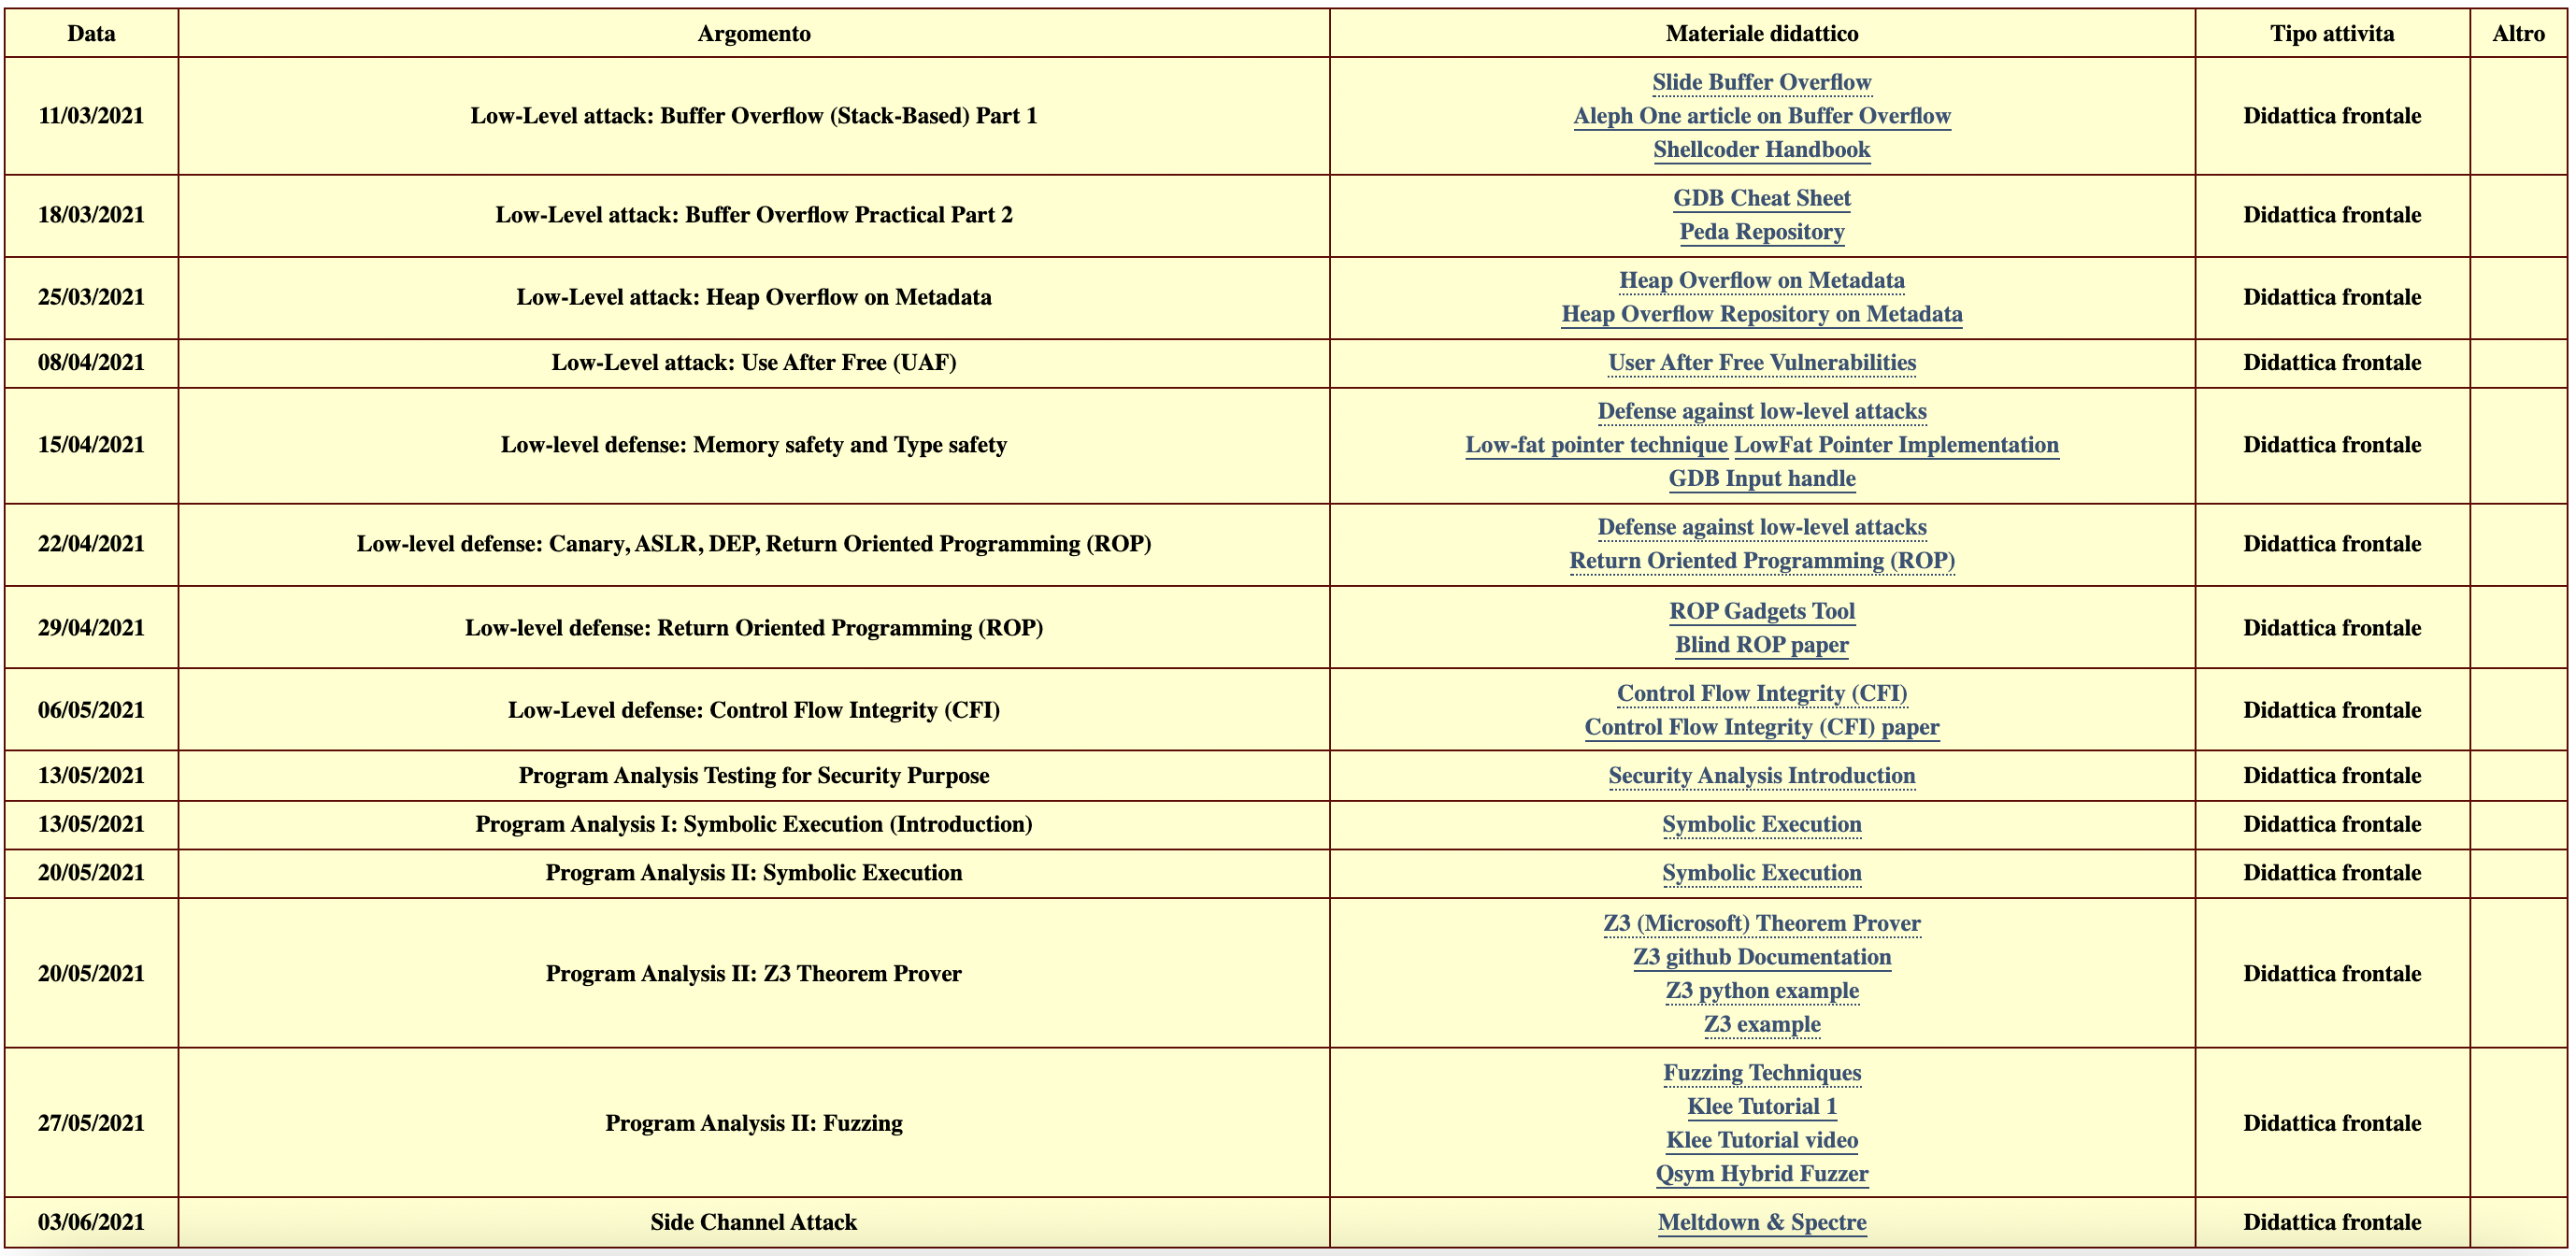
\includegraphics[scale=0.3]{programma}
%\subsection{}
\\\\
\textbf{Buffer overflow}\\
A buffer overflow is a bug that affects low-level code, normally a program would crash but an attacker can alter the situation \emph{to steal informations, corrupt valuable information or run an attacker's code of choice.}\\
They are relevant because C and C++ are still popular, and buffer overflow attacks stil happen regularly.
They have a long history and there are many approaches to defend against them.\\
There levels in which we can act to defend against them, the compiler, the OS, or the architecture.\\\\
\textbf{Memory Layout (32bit, Linux)}\\
In pile in a 32 bit system, Linux or Intel 32-bit the addresses range from 0x00000000 to 0xBFFFFFFF.\\
The stack, which grows downwards, is the place in which activation records are stored, together with the heap they are created in runtime. The heap is managed with malloc, calloc, free and grows upwards, and contains variables. The text segment contains the instructions.\\
\begin{center}
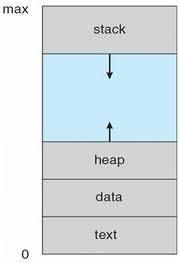
\includegraphics[scale = 0.5]{heapstack}
\end{center}
Memory operations make the memory grow upwards, this makes overwriting the SFP possible, allowing memory errors.\\
\begin{center}
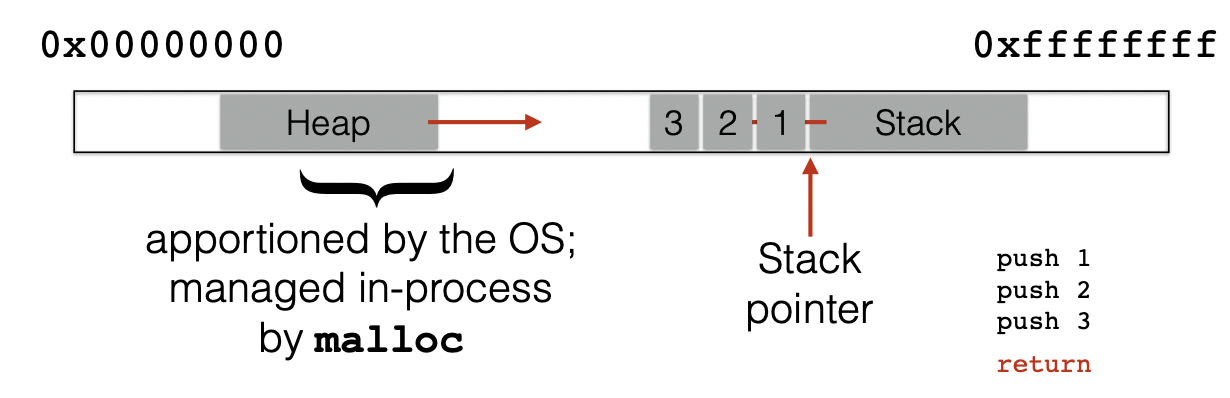
\includegraphics[scale = 0.5]{memory5}
\end{center}
\begin{center}
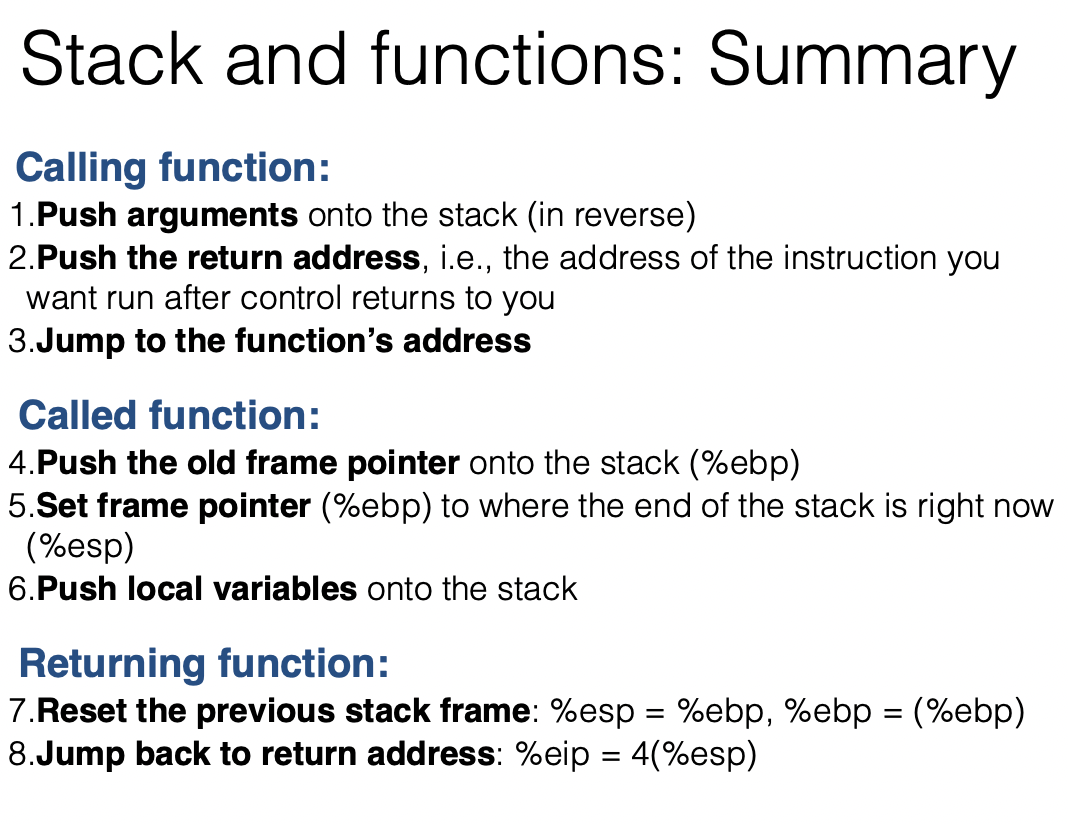
\includegraphics[scale = 0.4]{memory6}
\end{center}
Firstly let's talk about buffers, buffers are a contiguous piece of memory associated with a variable or a field, these are common in C. By overflowing a buffer we can put more into the buffer than it can hold.\\
In this example: BUF1 (which is big [24], is copied into BUF[20], since memory operation increases the heap upwards, it is possible to overwrite the SFP, causing a segmentation fault error.
\begin{center}
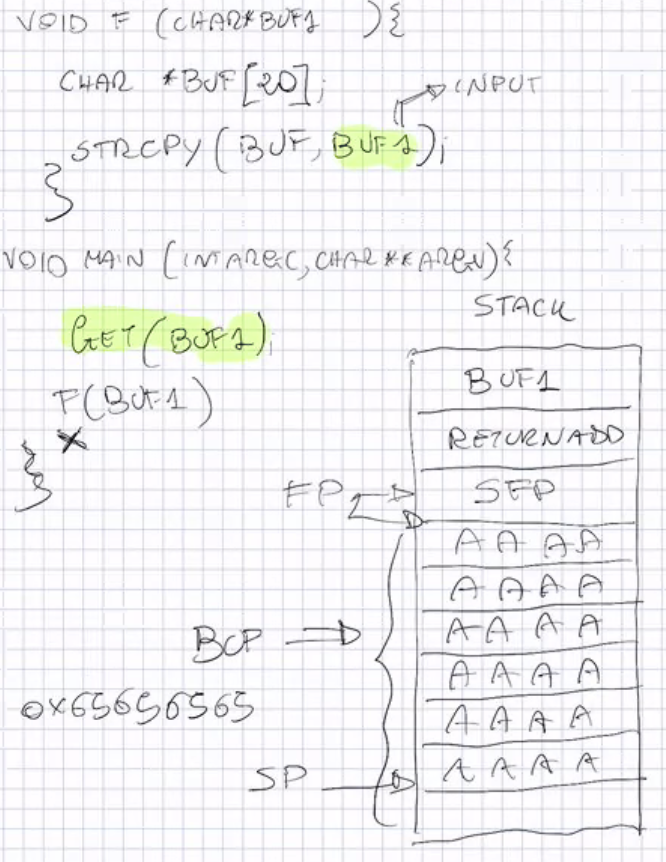
\includegraphics[scale = 0.5]{memory2}
\end{center}
Now we have crashed the system, but how can we exploit this?\\ 
Note that strcpy will let you write as much as you want till a terminator character, we could introduce particularly crafted code to wreak havoc.\\
If instead of AAAA (which is: 0x65656565) we introduce code which alters the normal execution of the program, overwriting the return address.\\
How do we build the injection vector?
\begin{center}
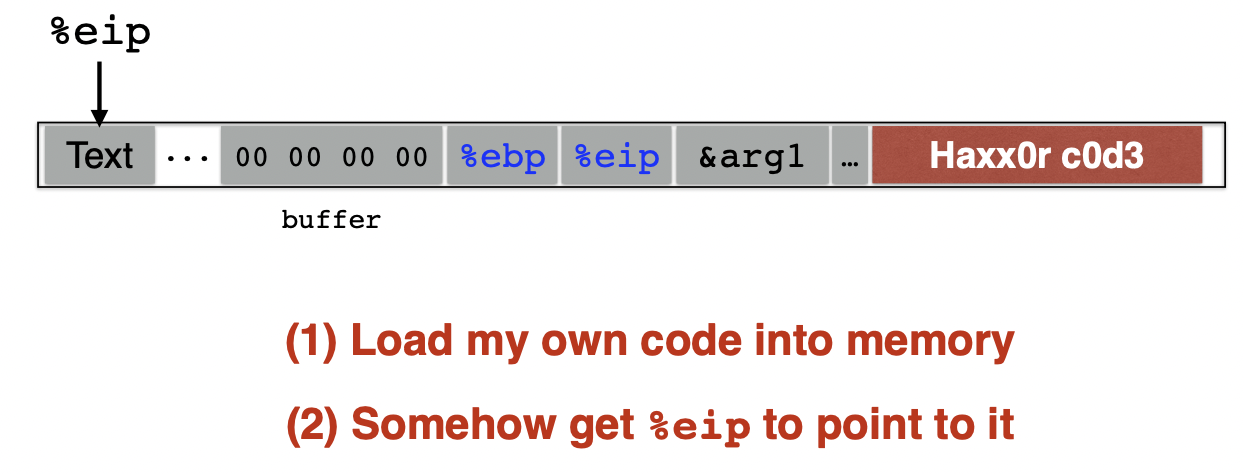
\includegraphics[scale = 0.4]{injcode}
\end{center}
{\footnotesize Note that the "disallocation" only consists in a subtraction of the reference pointer, the data remains\\
We introduce arbitrary shellcode, and by hijacking the return address we can execute code we want}\\
We can only load machine code into memory, which are instructions already compiled and ready to run, since we're trying to give the attacker general access to the system, the best candidate is the general-purpose shell. \\The shellcode is carefully crafted in the format \emph{[SHELLCODE][ADDRESSBUF] = Attack Vector} and it is copied with the function call "strcpy".
It is fundamental we get to know the [ADDRESSBUF], since if we don't an unrecognized instruction is going to run and C is gonna throw an IllegaArgumentException.\\
{\footnotesize Shellcode: machine code -that we want to execute- to run a shell}\\
The idea: we can't insert a "jump to my code" instruction, so we hijack the saved \%eip. Since we don't know the desired \%eip address we'll have to:\\
- Try a lot of different values, upwards of $2^{32}$ possible answers\\
- Without address randomization, the stack always start from a fixed address, and it doesn't grow very deeply.\\
How do we increase the chances to execute our shellcodes ?\\
Introduce the NOPSLED: 0x90 is a NOP instruction, single byte instruction which does nothing.
We can fill our vector buffer of NOP operations, thus increasing the chances of execution
\begin{figure}
\begin{subfigure}{0.4\linewidth}
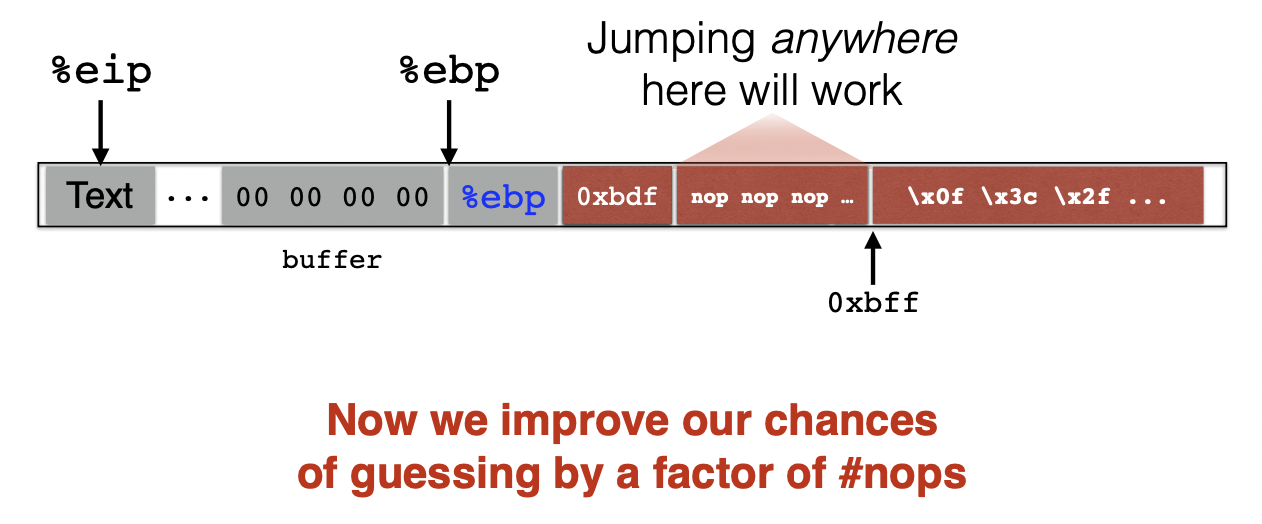
\includegraphics[width=\linewidth]{nop}
\end{subfigure}
\hfill
\begin{subfigure}{0.4\linewidth}
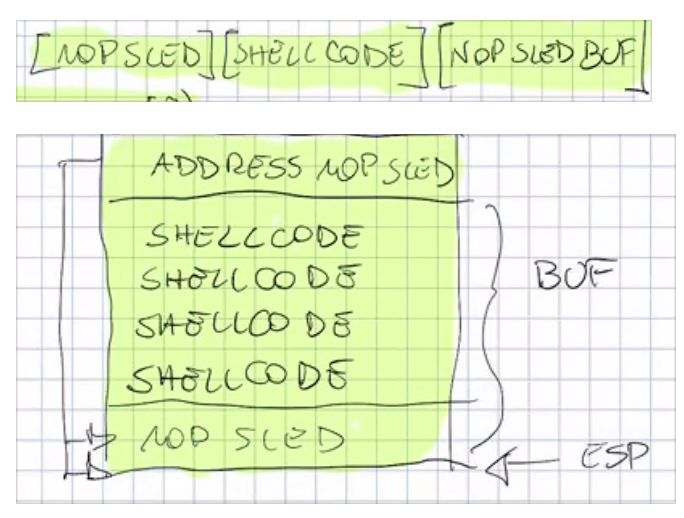
\includegraphics[width=\linewidth]{nopsled}
\end{subfigure}
\end{figure}
Depending on the size of the buffer, we have to size our shellcode. The size depends on the allocated space by the target char array in strcpy.\\ \emph{char BUF[20]; strcpy(BUF, BUF1); size of the buffer to work with is 20}\\\\
The computer by itself has protections, mainly towards the \textbf{returnAddress}, such as canary, nx\\\\

\emph{Heap vs Stack}\\
Let's take an overlook over the differences between the Stack and the Heap:
\begin{itemize}
\item The stack:\\
- has a fixed memory allocation, which is only known at compile time.\\
- inside it reside local variables, return addresses, functions args.\\
- it's very fast and automatic, and it is managed by the compiler.
\item The Heap:\\
- has dynamic memory allocation, known at runtime.\\
- inside it reside objects, big buffers, structs, persistence and larger objects\\
- it's slower, manual, managed by the programme
\end{itemize}
The Heap is a pool of memory used to dynamic allocations, managed with:\\
- \emph{malloc()}: to allocate memory on the heap\\
- \emph{free()}: to release memory on the heap\\\begin{center}
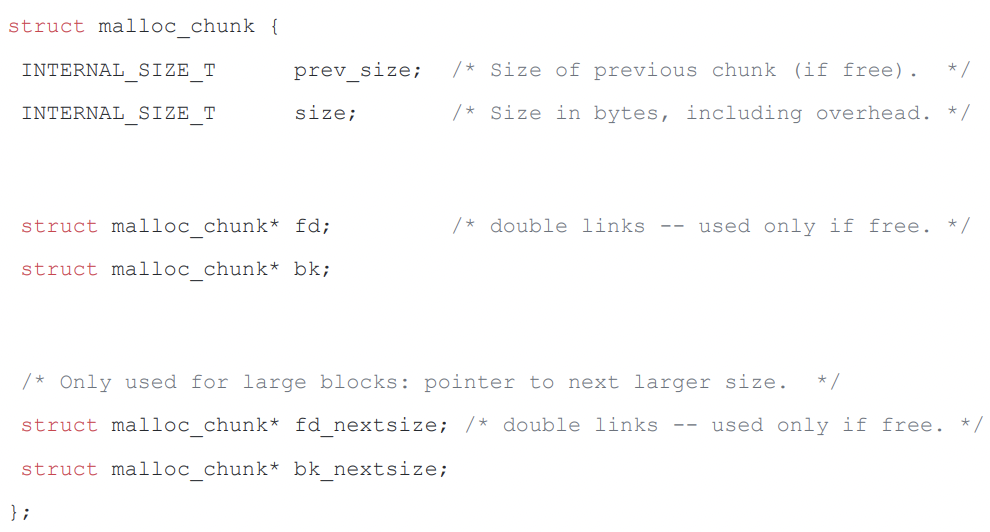
\includegraphics[scale = 0.6]{heap}
\end{center}
Let's see an overview of a heap chunk:
\begin{center}
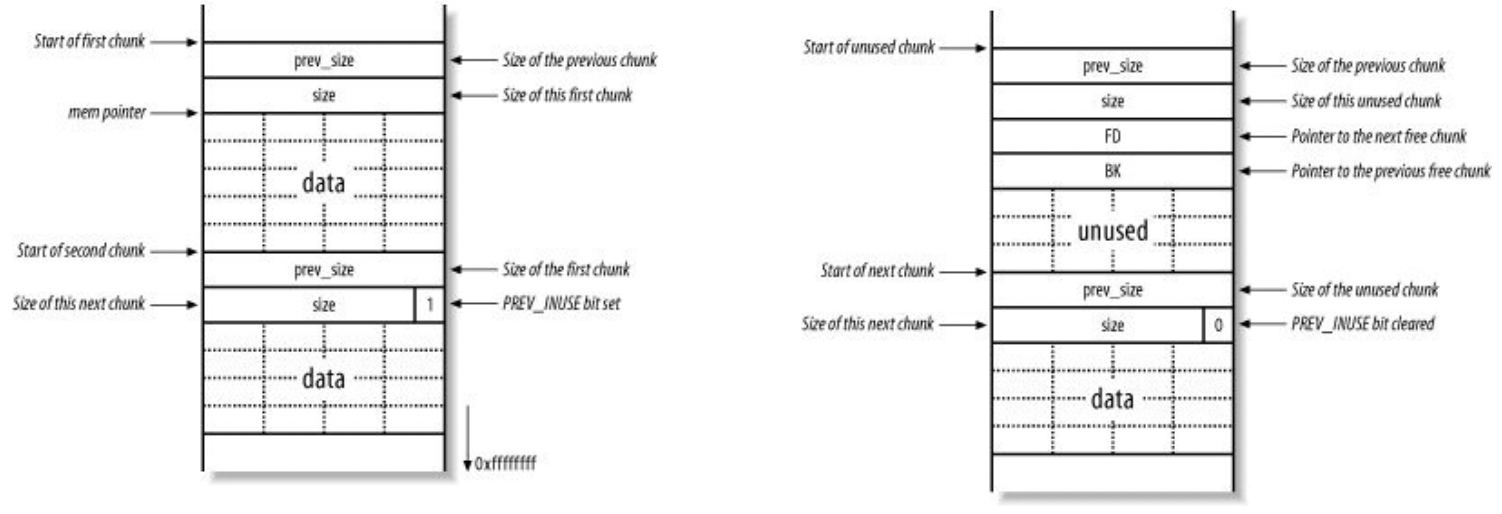
\includegraphics[scale = 0.6]{heap2}
\end{center}
The chunk is a part of the memory allocated in the heap. Alongside the data, it also contains metadatas:
\begin{itemize}
\item prev\textunderscore size: contains the size of the pervious chunk 
\item size: it is also equipped with a bit-switch \emph{PREV\textunderscore INUSE}.
It contains the size of the previous chunk.
\item FD: the pointer to next free chunk
\item BK: the pointer previous free chunk
\end{itemize}

The heap grows upwards.
\emph{prev\textunderscore size and size} concurrently form the metadata section of the heap chunk.
When we call \emph{P = malloc(128)}, the pointer points to memPointer, just below the metadatas.\\\\
\emph{The free function}
When \emph{free(p)} is used, the LSB of the size field in the metadata of the next chunk is cleared. Additionally the prev\textunderscore size field of the next size will be set to the size of the chunk we are currently freeing. \\
The system keeps multiple lists of the freed chunks, which can be of different size, when a chunk is freed, we can verified if the previous chunk is freed to, and if it is we can unify them into a single bigger chunk.\\
When an allocation request is made, the system looks into the first free chunk that has a size \(\geq\) than the size requested. If no free chunk is found, the top chunk will be used.\\\\
AV\textunderscore TOP è il riferimento al top chunk; rappresenta lo spazio rimanente. Quando solleviamo una memory request e lo spazio nello heap è esaurito \emph{eg. malloc(256)} il topchunk è diviso in due, e rispettivamente le parti diventano topchunk e la parte richiesta.\\
When we deallocate a chunk, we use an unlink function, this leaves an opening for us, the attacker. By hijacking the two metadata values it allows us to write an arbitrary value to an arbitrary location.
\begin{center}
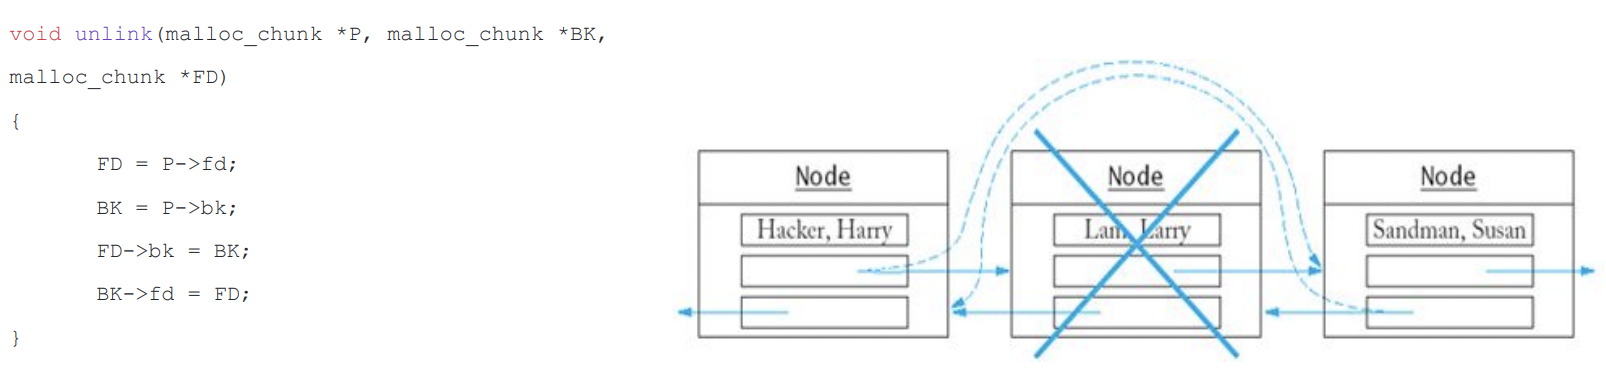
\includegraphics[scale = 0.6]{atk1}
\emph{the intended process}
\end{center}
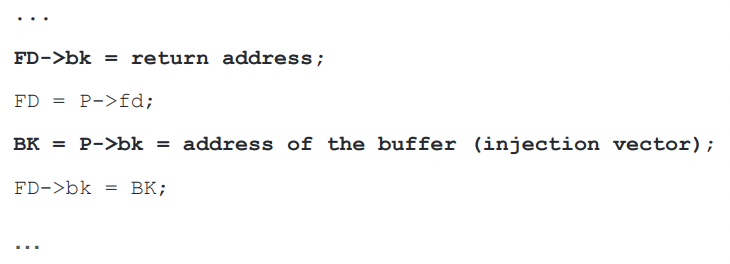
\includegraphics[scale = 0.6]{atk2}
\begin{center}
\emph{malicious code which allows us to manipulate the BK}
\end{center}
Unfortunately this technique no longer works, the current unlink function verifies beforehand the values
We can however look for other flaws:\\
\emph{House of Force vulnerabity}
Conditions:
\begin{itemize}
\item It requires 3 malloc, more precisely a malloc that allows us to overwrite the top chunk, one malloc with a user controllable size and another call to malloc.
\item 1 (or 2) strcpy
\end{itemize}
\emph{Use after free vulnerability}
Use after free vulnerability are vulnerabilities that happen when a  pointer to an object that hash been freed is deferenced. This can lead to information leakage, and furthermore the attacker could also modify unintended memory locations that can potentially lead to code execution.\\
A prime candidate for an attack is a dangling pointer. Dangling pointer happen when a pointer, which was previously the target of another pointer is deleted, leaving the other pointer dangling.\\
\begin{center}
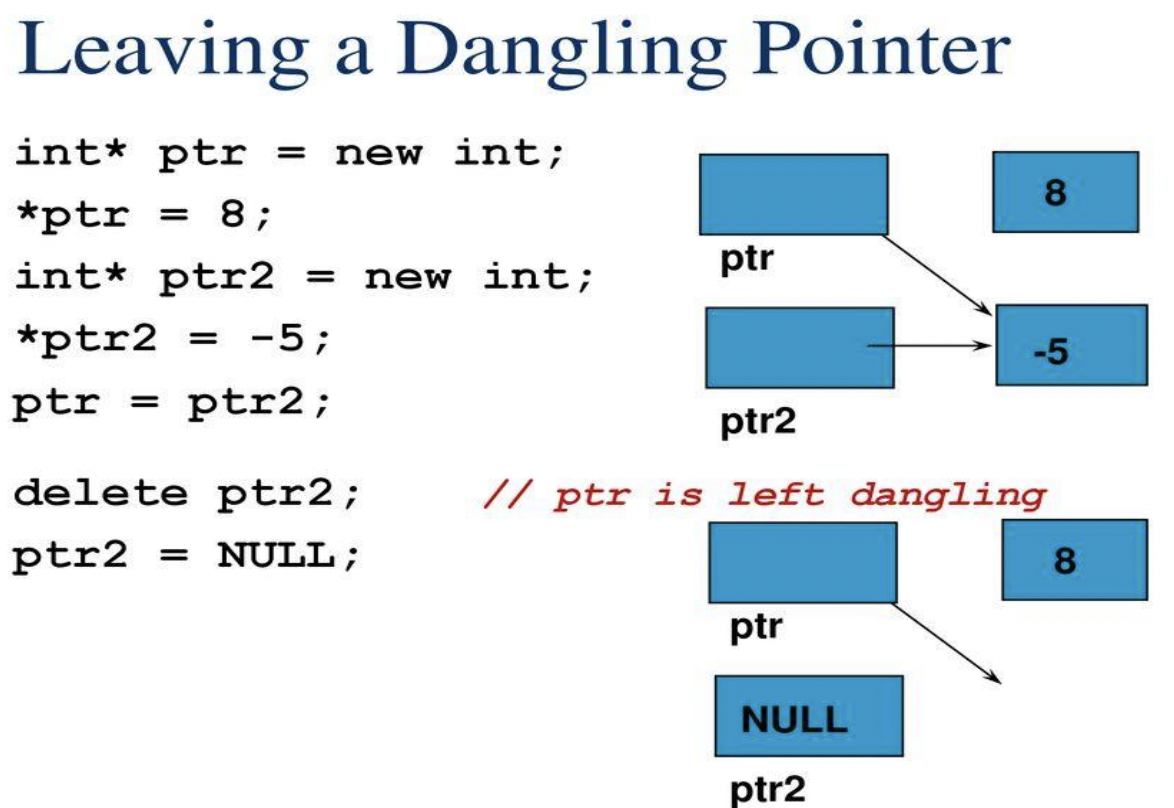
\includegraphics[scale = 0.6]{dpointer}
\end{center}
This happens because in C the entire management of pointers is left to programmers. In java this issue doesn't manifest itself because unused/unallocated memory spaces are collected by the garbage collector.\\\\
Let's see an actual example of user after free vulnerability
\begin{center}
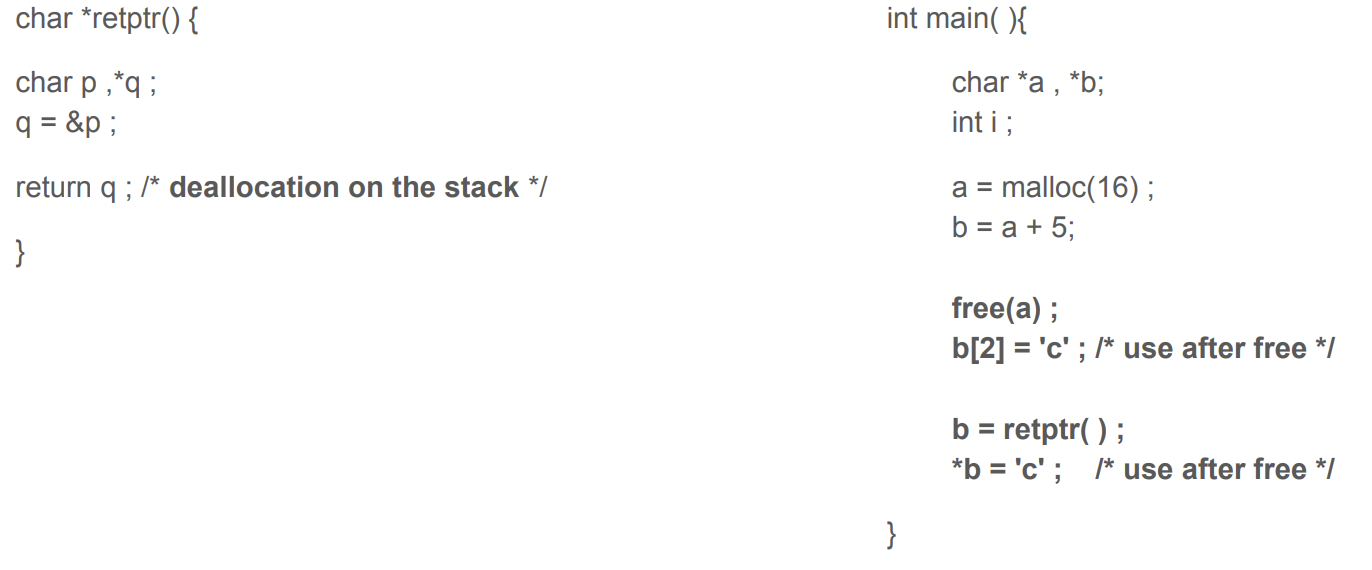
\includegraphics[scale = 0.6]{usafter}
\end{center}
In this example, a is a contiguous memory space long 16 bytes, b points to a location inside of a.\\
b, after using \emph{b[2] = 'c'} is able to modify a memory portion of a after it has been freed (de-allocation).
\begin{center}
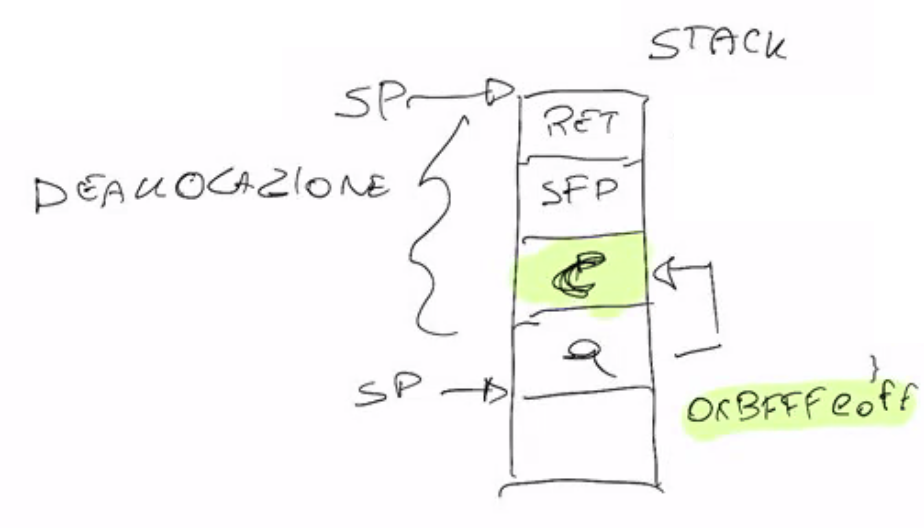
\includegraphics[scale = 0.6]{usafter2}
\end{center}
b punta a una porzione dello stack che è stata deallocata. chiamando *b = 'c' modifichiamo una porzione dello stack che è stata deallocata precedentemente (nello stack p diventa c).
\\\\\\

\emph{Defence and mitigation mechanisms}\\
All these attacks have in common a couple of characteristics:\\
- The attacker is able to control some data that is used by the program\\
- The use of data permits unintentional access to some memory area in the program past a buffer, or to an arbitrary position on the stack.\\
So what can we do to \emph{mitigate} these vulnerabilities?\\
First of all it's important we mention that we are not going to implement solutions which are going to leave us with a type safety and memory safety language. We are only going to implement mechanisms which are going to make the exploitation of these vulnerabilities too costly/time consuming.\\\\
Type safety and memory safety are two fundamental mechanisms which can help us mitigate these vulnerabilities, these properties, if met, ensure an application is immune to memory attacks. Languages such as C and C++ don't implement memory and type safety due to its efficiency load, other languages that do are JAVA or Python.\\\\
\emph{So what can we actually do?}
\begin{itemize}

\item Automatic defences:\\
these defences are specific to the compiler and help protect the return address and
- Stack canaries: protects the return address from hijacking.\\
More precisely a stack canary is a value placed on the stack such that a stack-buffer overflow will overwrite it before corrupting the return address. The buffer overflow can then be detected by verifying the integrity of the canary before performing the return. It is fundamental that the stack canary remains confidential, otherwise the attacker could just copy it and hijack the control flow anyway
\begin{center}
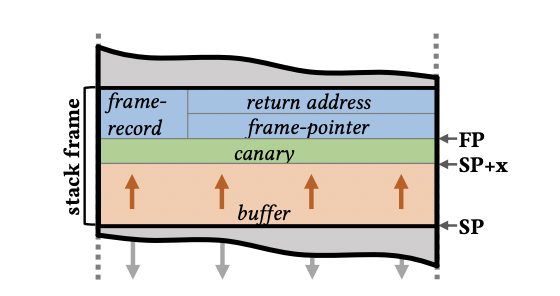
\includegraphics[scale = 0.6]{canary}
\end{center}
- Address space layout randomisation \textbf{(ASLR)}: is a memory-protection process for operating systems that guards against buffer-overflow attacks by randomising the location where system executables are loaded into memory. \\Being able to determine beforehand the position of processes and functions in memory makes exploitation easier, and ASLR is able to put address space targets in unpredictable locations, the attacker won't be able to identify the correct address space, making the application crash and notifying the system.
\item Return-oriented programming \textbf{(ROP)}attacks are based on the technique that allows the attacker to hijack the program control flow by executing machine code instructions present in the machine's memory. \\
This is done by manipulating the call stack by exploiting vulnerabilities in a program, typically a buffer overflow.\\
Control Flow Integrity \textbf{(CFI)} are mechanisms implemented to prevent a variety of attacks based on the redirection of the control flow of the program.
\item Secure coding are a set of practises that applies to security considerations that help defend against vulnerabilities, bugs and exploits. Secure coding introduces safeguards which reduce or eliminate the risk of leaving security vulnerabilities in the code, most important of which are \textbf{memory safety and type safety}
\end{itemize}

\emph{Memory Safety}
Memory safety is a fundamental principle which helps mitigate 
To guarantee a degree of memory safety in C we can:
\begin{itemize}
\item only create pointer through standard means
\begin{center}
p  = malloc(...), or p = \&x, or p = \&buf[5] etc.
\end{center}
item only use pointers to access memory that "belong" (that is withint the bound) of that pointer and of the type that corresponds. (int* to integers, char* to characters).
\end{itemize}
This essentially combines two principles: \emph{temporal safety and spatial safety}.


\textbf{Spatial Safety} (in the heap)\\
Let us 
Pointers are viewed as triples $(p, b, e)$ where:
\begin{itemize}
\item $p$ is the actual pointer
\item $b$ is the base of the memory region it may access
\item $e$is the extend (or the bounds) of the region
\end{itemize}
The deferenced access shall be allowed iff $ b \leq p \leq e - sizeof(typeof(p))$. 

An implementation of a spatial safety compliant memcpy
\begin{center}
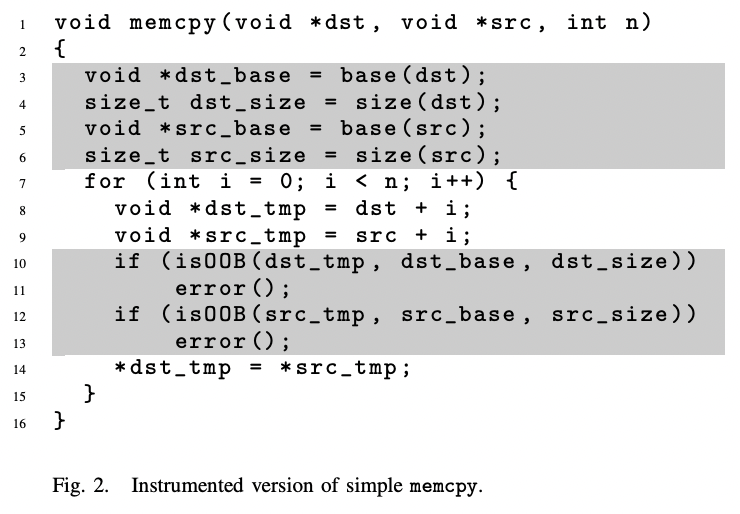
\includegraphics[scale = 0.6]{memsef}
\end{center}


\textbf{Temporal safety}\\
Memory regions can either be defined or undefined:\\
- defined means allocated (and active)\\
- undefined means allocated, uninitialised, or deallocated\\
A temporal safety violation occurs when an attacker tries to access undefined memory space\\ 
- spatial safety assures that an accessed region is legal\\
- temporal safety assures that region is still in play\\\\
When a free function is called, the pointer towards that region is freed up, but the data remains in the stack, just unreferenced. The garbage collection's job is the memory management, its main function si to reclaim memory which was allocated by the program, but is no longer referenced.\\
The aim is to implement mechanisms similar to the garbage collector, but not quite; we want to protect vulnerable portions of the memory. The garbage collectors are demanding in terms of resources.\\\\
But why would we want to use a language that is \textbf{not memory safe and type safe}?\\
The easiest way to avoid all these vulnerabilities would be to use a \textbf{memory safe language}, languages that are \textbf{type safe are even better.} 
\begin{center}
\textbf{Type safety  $>$ Memory Safety}
\end{center}
The main reason is that C and C++ are \textbf{here to stay}, while not memory safe, writing memory safe programs is possible.\\The problem of type safety and memory safety has been known for more than 20 years, the limiting factor has always been \textbf{performance}  (around 12x and 17x overhead). Furthermore adding type safety would also make C and C++ much slower. \\
Type safety enforcement is expensive, the most important mechanisms are 
\begin{itemize}
\item \textbf{Garbage collection} which avoids temporal violations, but uses much more memory
\item \textbf{Bound} and null pointer checks which avoids spatial violations
\item \textbf{Hiding representation} may \textbf{inhibit optimisation}\\
technique such as C-style casts, pointer arithmetic, \& operators would not be allowed
\end{itemize}
\emph{So what can we do in C?}
\begin{itemize}
\item Compiler could add code to \textbf{check for violations}\\
An out-of-bounds access would result in immediate failure just like an \emph{ArrayBoundsException} in Java.
\item \textbf{No dangling pointers}\\
Accessing a freed pointer violates temporal safety, accessing uninitialised pointers is also not OK:
\begin{figure}[H]
\begin{subfigure}[H]{0.5\linewidth}
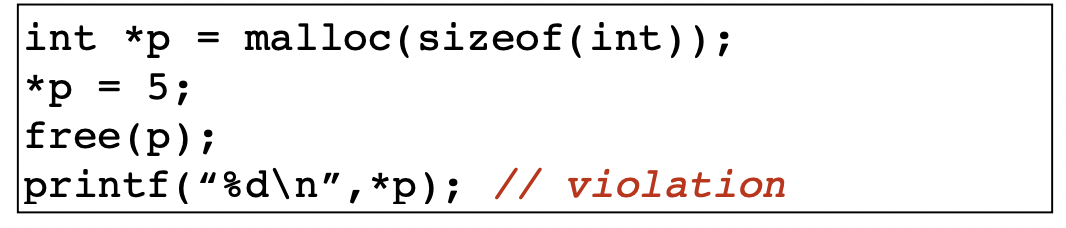
\includegraphics[width=\linewidth]{sef1}
\end{subfigure}
\begin{subfigure}[H]{0.5\linewidth}
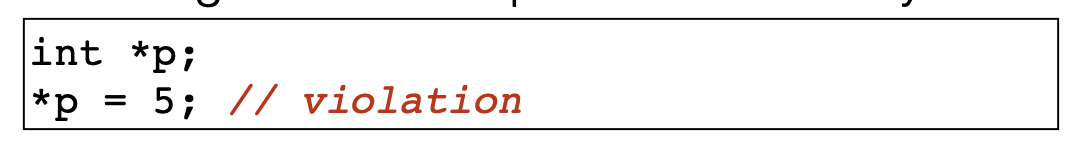
\includegraphics[width=\linewidth]{sef2}
\end{subfigure}%
\end{figure}
\item \textbf{Type safety}\\
Each objects shall be ascribed a type (int, pointer to int, pointer to function).\\
Operations on he objects shall be always compatible with the object's type. Type safe programs can't encounter runtime errors. Type safety implies that objects shall always have a compatible types, while guarantee bounds compliance
\begin{center}
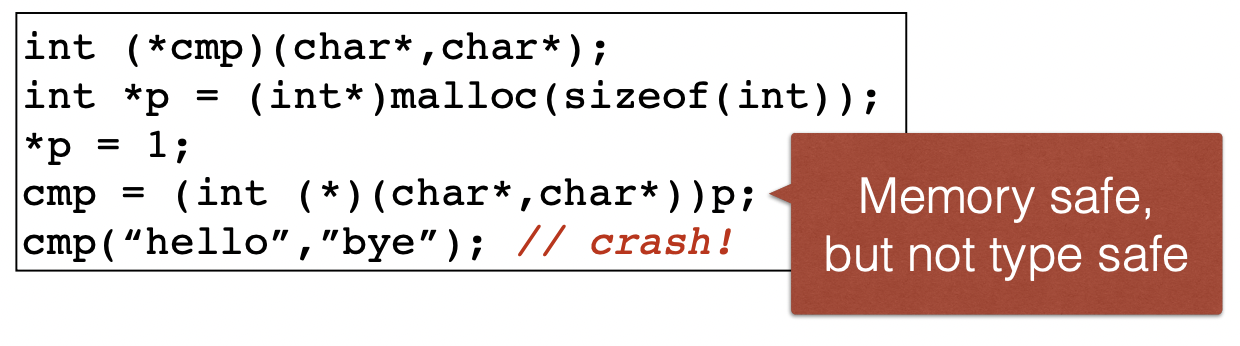
\includegraphics[scale = 0.6]{tsef}
\end{center}
So how can we guarantee a degree of type safety in C?
Using \textbf{enforce invariants}, are properties which cannot be violated by type, by enforcing invariants in the program. Most notably is the enforcement of \textbf{abstract types}, which characterised modules. It keep the \textbf{representation of the modules hidden from others}. This guarantee a \textbf{degree of isolation} from the rest of the system.\\\\
Type-enforced invariants can relate to security properties, by expressing stronger invariants about data's privacy and integrity we can mitigate type mismatch exploits, such as the following in Java.
\begin{center}
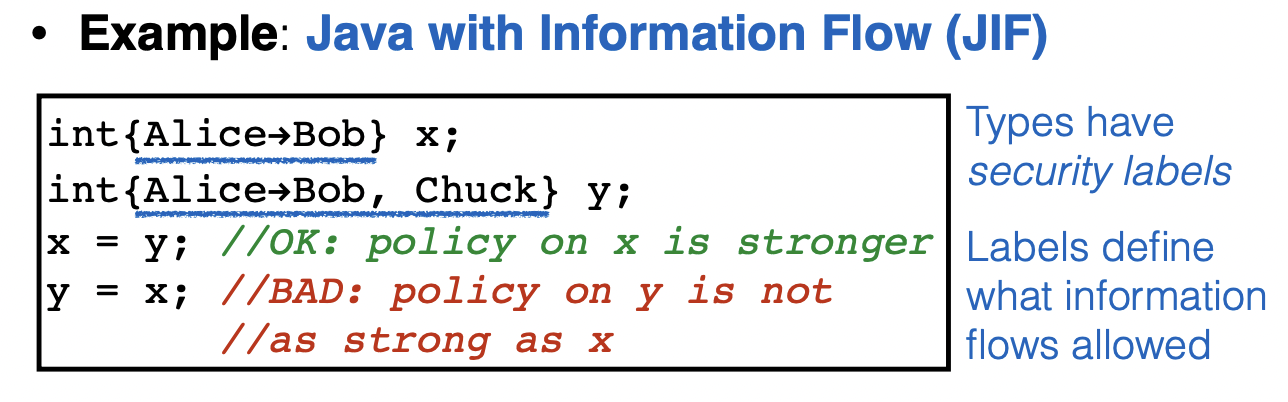
\includegraphics[scale = 0.6]{alice}
\end{center}
All of these mechanisms concurrently compose the security by design principle, which means that the language and its capabilities are foundationally secure. In this approach security is built into the system, not mitigating since the design stage notable vulnerabilities.\\
There are already languages which provide similar features to C, while remaining type safe, notable examples are Google's Go, Mozilla's Rust, Apple's Swift.
\end{itemize}
\textbf{Other defensive strategies:}\\
These are complementary, they mitigate bugs but can't shut them out entirely
\begin{itemize}
\item Make the bug harder to exploit: introduce more steps, to make them difficult or impossible
\item Avoid the bug entirely: practice secure coding practices, advanced code review and testing
\end{itemize}
To implement these, let's recall the steps of a stack smashing attack:
\begin{itemize}
\item Putting the attacker code into the memory. The shellcode must also not contain zero (it is interpreted by the machine as a string terminator)
\item Getting \emph{\%eip} to point at the shellcode
\item Finding the return address (by guessing the raw address)
\end{itemize}
To make these attacks steps more difficult we can use libraries, compiler mechanisms and the operating system. We are trying to fix the architectural design, and not the code.
\section*{Overflows detection using canaries:}
Managed by the compiler, canaries work by protecting the return address by detecting any change that could have harmed the stack's integrity. The canaries are placed inside the stack in a protected memory section between user and system variables. \\The canary's value has to be random, and unaccessible by the attacker otherwise it could be overwritten with the same value.
The canary is introduced when the function is called, using a machine code function called \emph{push canary}
\begin{center}
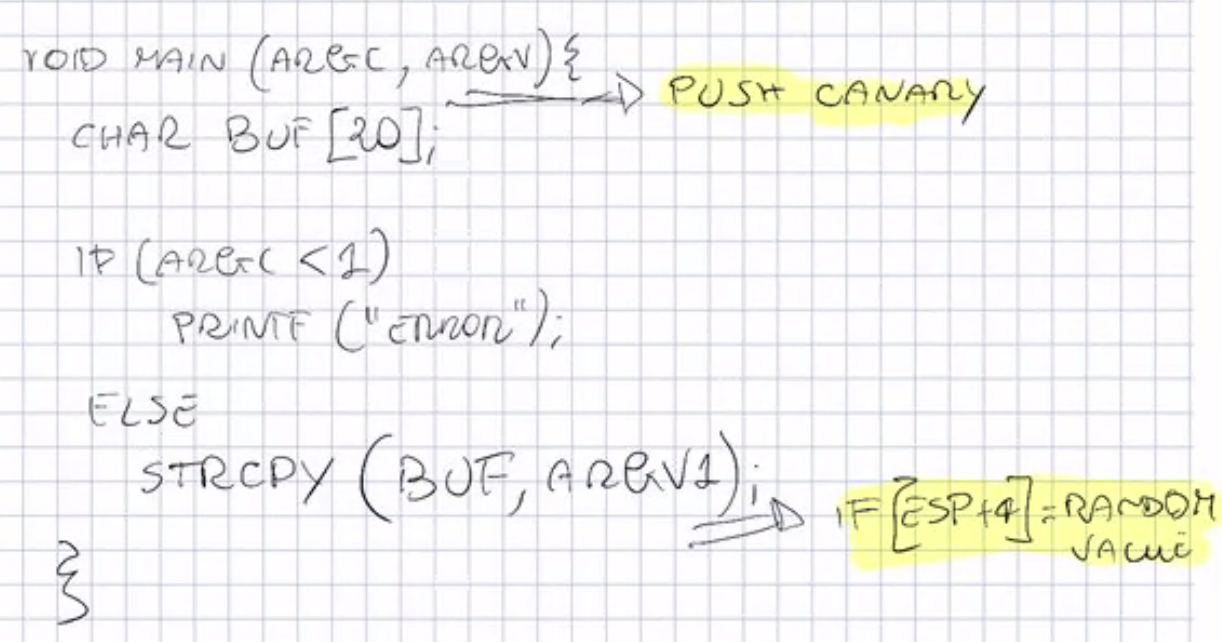
\includegraphics[scale = 0.6]{pushcanary}
\end{center}
Before calling the \emph{ret} the value of the canary is checked, raising errors if it's not correct.
The values the canary can assume are these:
\begin{center}
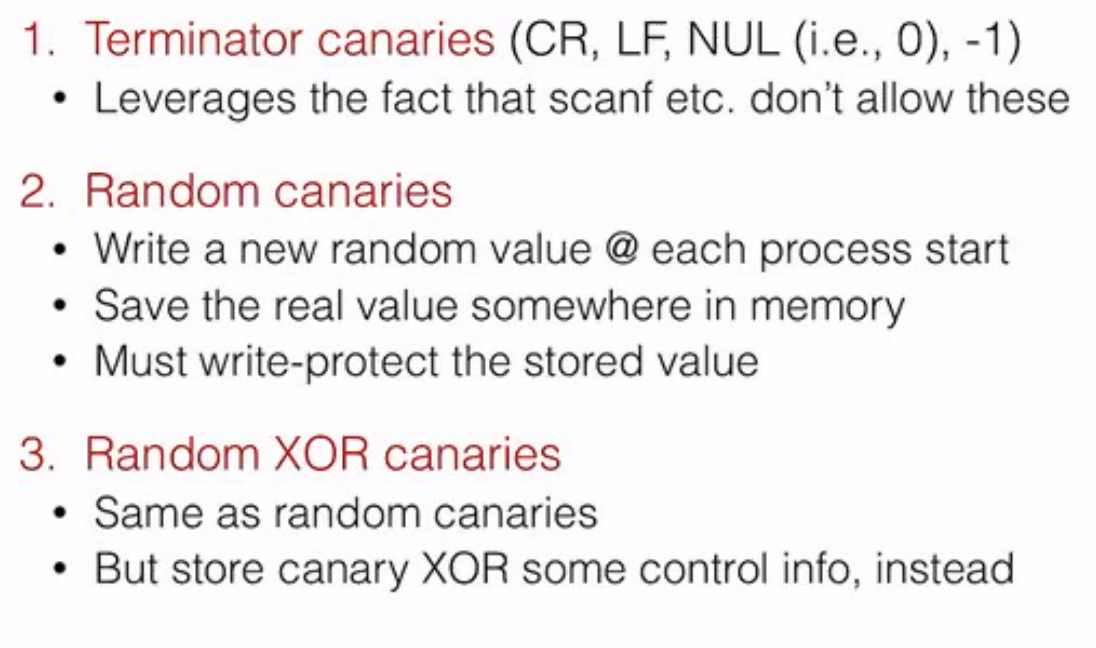
\includegraphics[scale = 0.6]{values}
\end{center}
3. Random XOR canaries work by doing:
\begin{enumerate}
\item $[ret$ $XOR$ $canaryValue]$ to produce che canary value
\item $[ret$ $XOR$ $canaryValue]$ the verify the canary value
\end{enumerate}
This works due to the nature of XOR, calling it two times gives us the initial value
\section*{DEP: Data Execution Prevention:}
This defence works by making the stack and heap memory space non-executable. Attackers bypassed this defence by having the shellcode point to system libraries in an attack called \emph{return-to-libc}.\\ lib-c libraries are used by the gcc compiler, meaning they are always available.\\\\
To use this attack, system is called. System is a function that has argument a terminal command. In order to work with this vulnerability, we need to first: call the system function, and two: have it run a meaningful command. This is done by placing the command next to the system call. The injection vector is modified in the following way.
\begin{center}
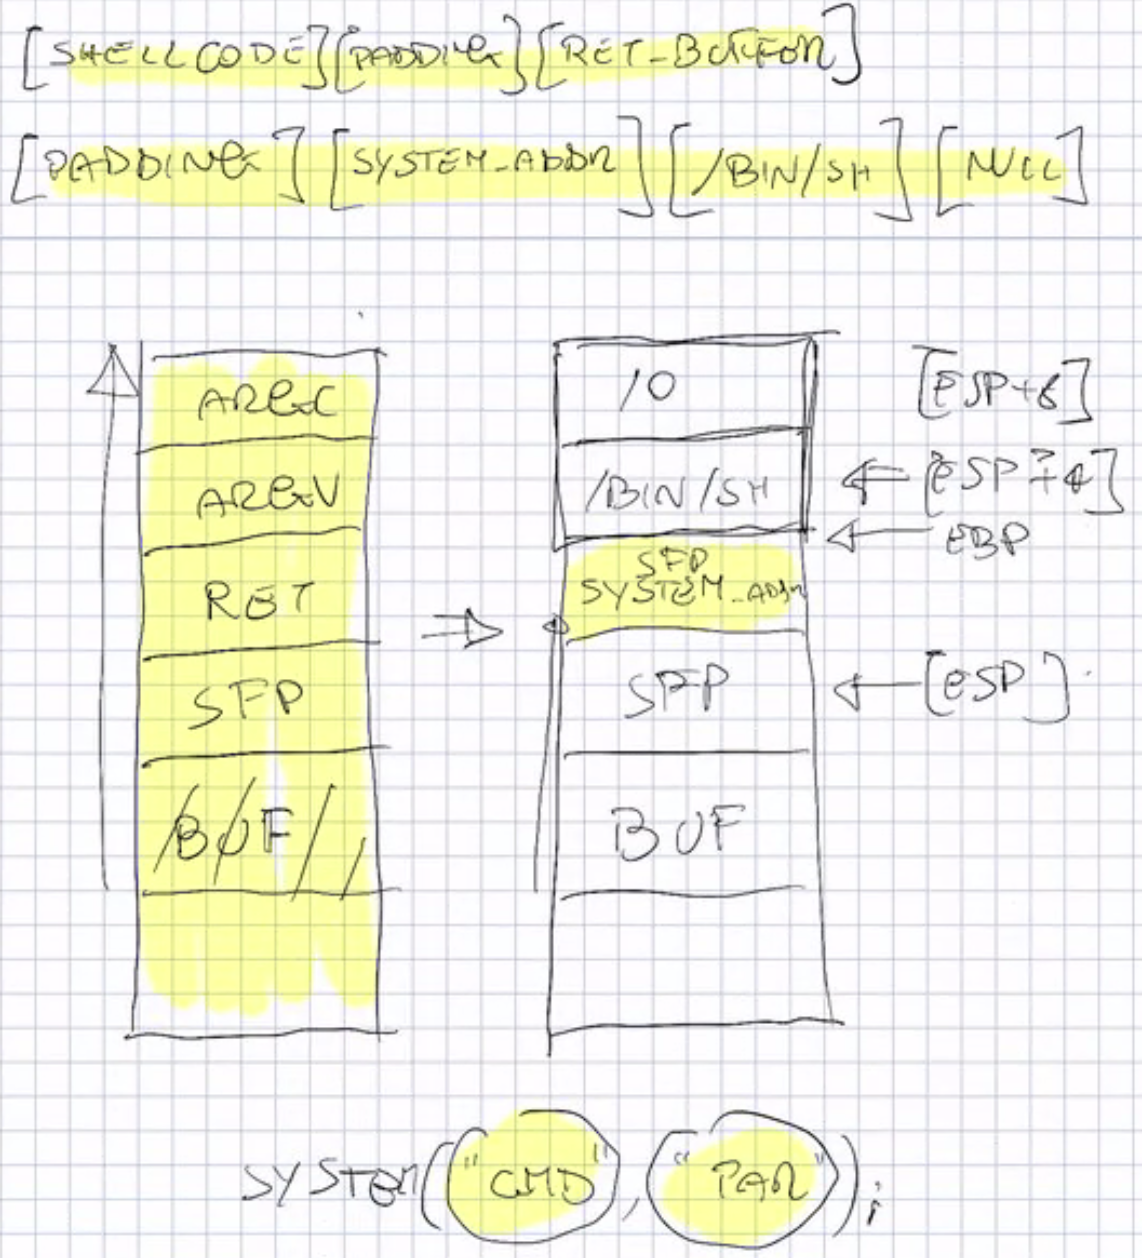
\includegraphics[scale = 0.5]{libc}
\end{center}
Defence strategies mitigated the \emph{return-to-libc attack} by introducing \emph{Address-space Layout Randomitazion or ASLR} which places standard libraries and other elements in memory in random places, making them harder to guess. It also has some caveats:
\begin{itemize}
\item Only shifts the offset of memory areas, not particular locations within those areas
\item May not apply to program code, but only libraries
\item Need sufficient randomness, otherwise it could be brute forced.\\
this makes this technique more promising on 64-bit systems
\end{itemize}
When we talk about \emph{cat and mouse} we mean the game of cat and mouse being played by attackers and the defence specialists.
\begin{center}
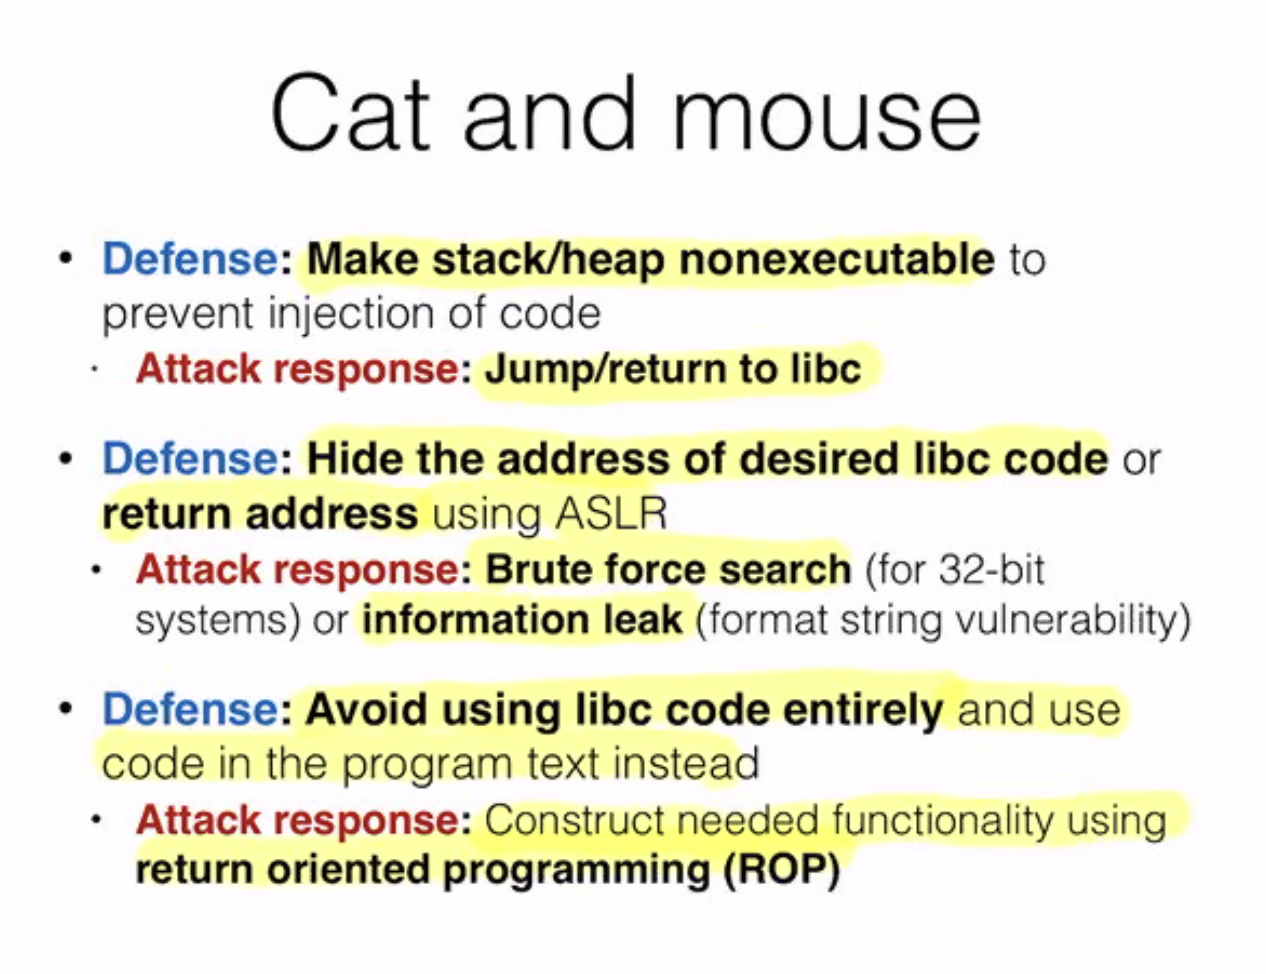
\includegraphics[scale = 0.5]{catmouse}
\end{center}
\section*{Return oriented Programming}
First introduced by Hovav Shacham in 2007, the idea is: rather than use a single libc function to run the shellcode, we string together pieces of existing code called gadgets to do it. Intuitively, we need to find the gadgets we need, and we need a mechanism to string them together\\\\
\textbf{gadgets}\\
Gadgets are instruction groups that end with \emph{ret}
\begin{figure}[H]
\begin{subfigure}[H]{0.2\linewidth}
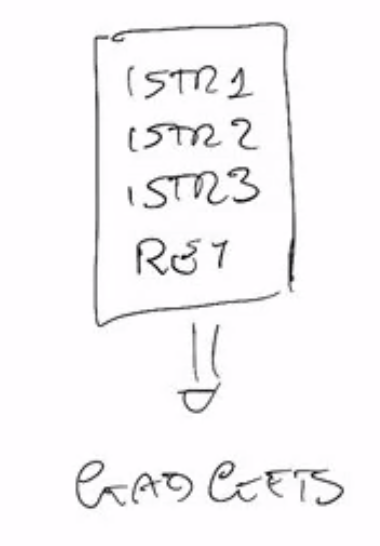
\includegraphics[width=\linewidth]{gadget}
\end{subfigure}
\hfill
\begin{subfigure}[H]{0.5\linewidth}
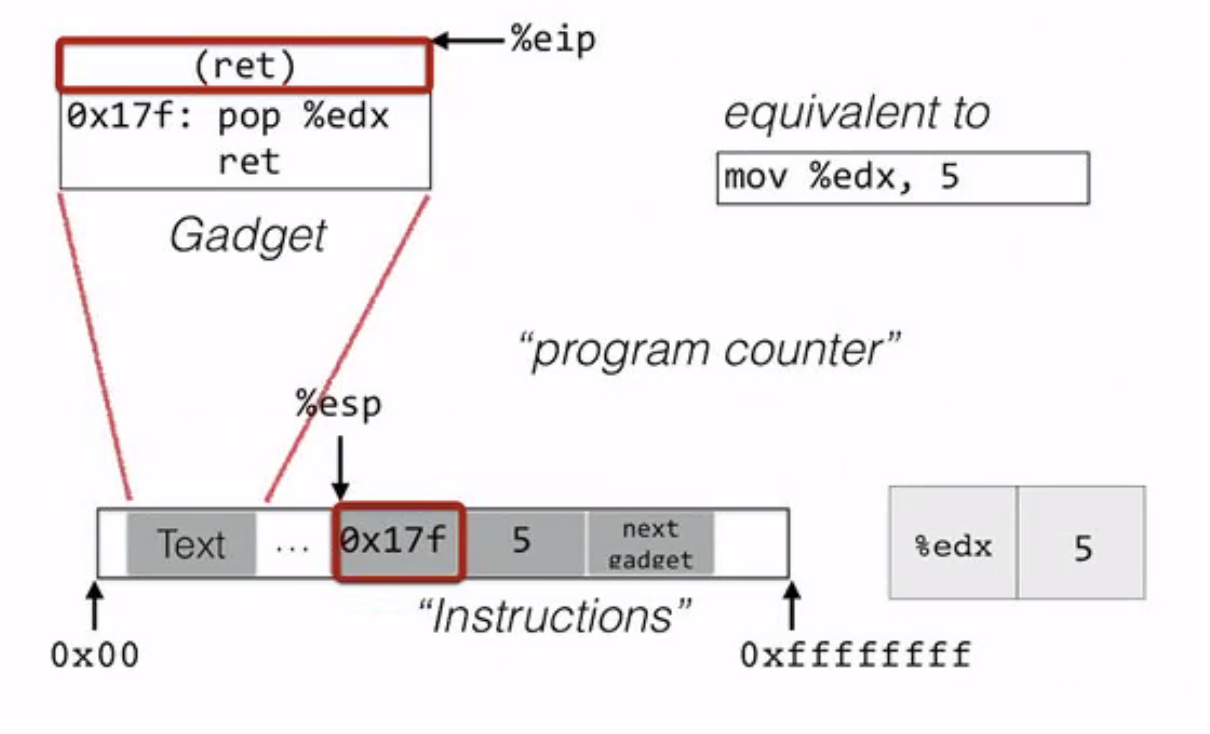
\includegraphics[width=\linewidth]{gadex}
\end{subfigure}%
\end{figure}
The memory structure that we're using is still the stack, which is also where we're loading our code.\begin{itemize}
\item \%esp serves as program counter
\item \emph{gadgets} are invoked via \emph{ret} instruction
\item \emph{multiple gadgets} are linked with each others using \emph{ret} instructions
\item \emph{gadgets} get their arguments via \emph{pop, peek etc.}
\end{itemize}
In this example we're trying to find an applicable instruction equivalent to \emph{mov \%edx, 5}, being: \emph{pop \%edx ret}.\\

\emph{So how do I actually find gadgets?}\\
One approach would be an automated search of the target binary for gadgets. This technique work by looking for \emph{ret} instructions, by working backwards.
\emph{Are these gadgets actually enough to do anything interesting?}\\
Yes, Shacham found that with significant codebases (such as libc) gadgets are \emph{Turing complete} meaning they're theoretically capable of solving any computational problem. Scwartz, in 2011, automated the gadget shellcode creation process (ROP compiler), without needing Turing completeness.\\\\
In CISC there is a degree of variability in the length of instruction (which is not present in ARM for example since it's a RISC)(RISC instruction lengths are fixed) which provides an extensive degree of freedom to exploits gadgets. This particular aspect is called dense Instruction Set.
\begin{figure}[H]
\begin{subfigure}[H]{0.4\linewidth}
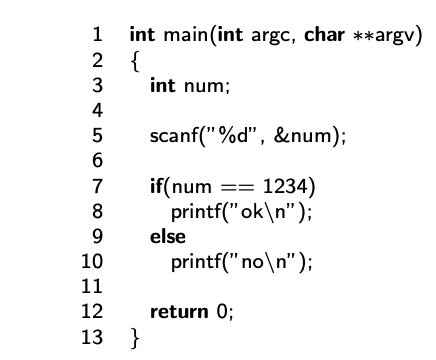
\includegraphics[width=\linewidth]{b1}
\end{subfigure}
\begin{subfigure}[H]{0.8\linewidth}
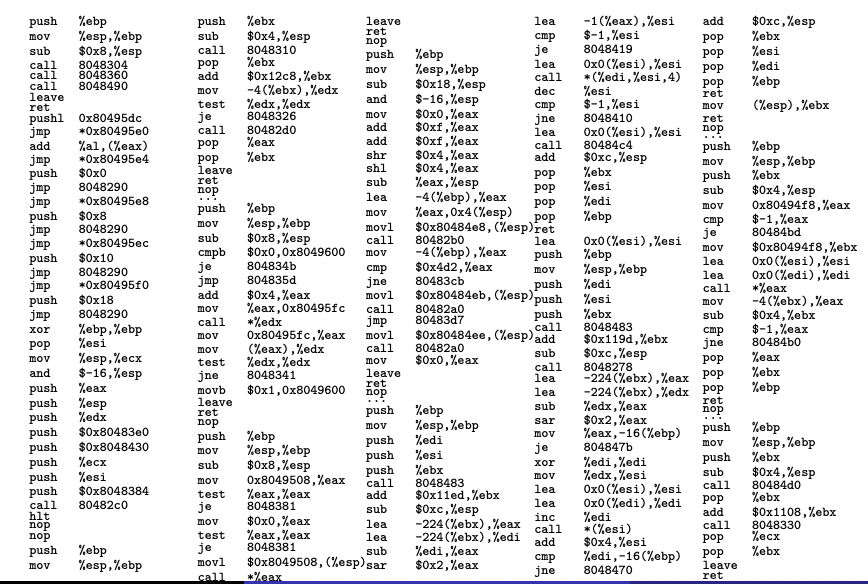
\includegraphics[width=\linewidth]{b2}
\end{subfigure}%
\end{figure}
With a simple program like this, we can extract a gigantic amount of instruction.
\section*{Hacking Blind}
Berkley students attack a victim server via a socket, which has all the defence mechanisms we have previously seen enabled, namely ASLR, canary and DEP. The attack happens based on a socket and a linux 64 bit server, via buffer overflow. The exploitation is based on the \emph{write} function:\begin{center}
\emph{write(SD, [buffer], length}\\
SD is soket descriptor
\end{center}
Utilising a flaw in the \emph{write} function the attacker is able to copy the buffer portion of memory
\begin{center}
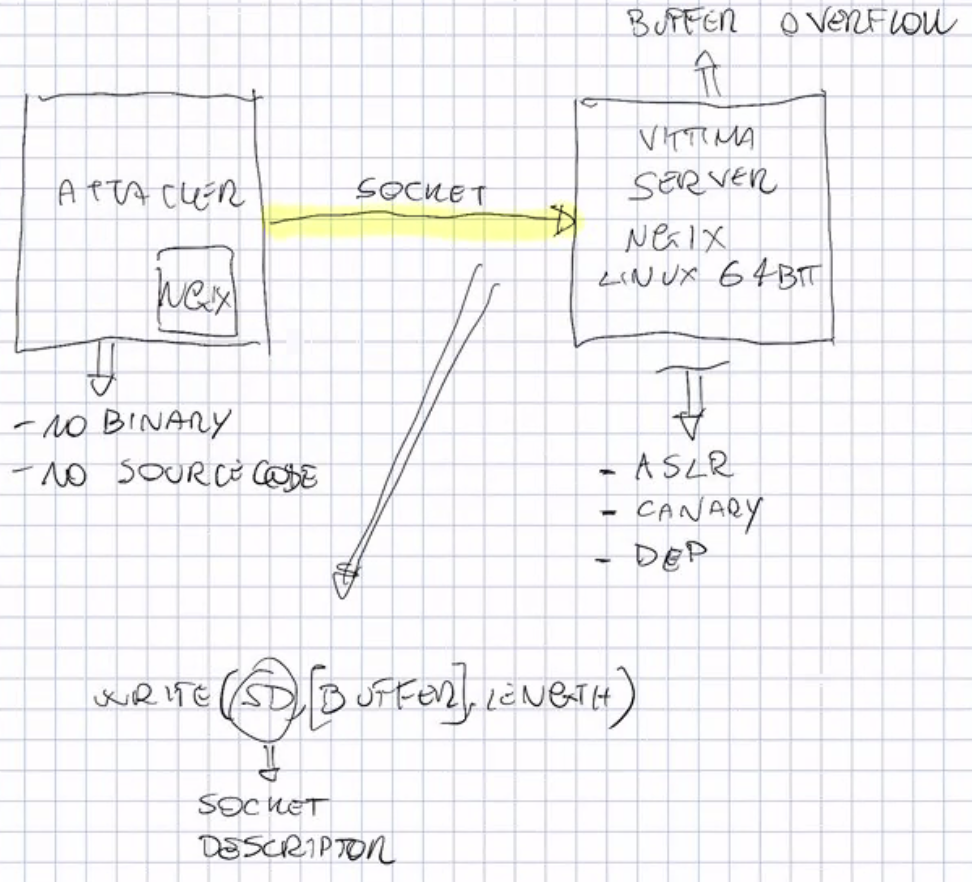
\includegraphics[scale = 0.5]{socket}
\end{center}
A fully automated attack based on this exploit yields a shell in under 4000 requests (20 minutes) against a modern system. \textbf{Techniques needed}:
\begin{enumerate}
\item Generalised stack reading: the possibility to read the stack in its entirety, used to leak the canaries (replace them with he correct values), and to defeat the ASLR (if I am able to read the stack, I am also able to read the location of the program).\\
Attacking canaries is based on the fact that when a thread crashes on a server, only the thread is reset, not the entire system, and therefore the canary stays the same. The attacker can progressively guess byte per byte the value of the canary. In this example the canary is of size 4 bytes, but on 64 bits system the canary is of size 8 bytes.
\begin{center}
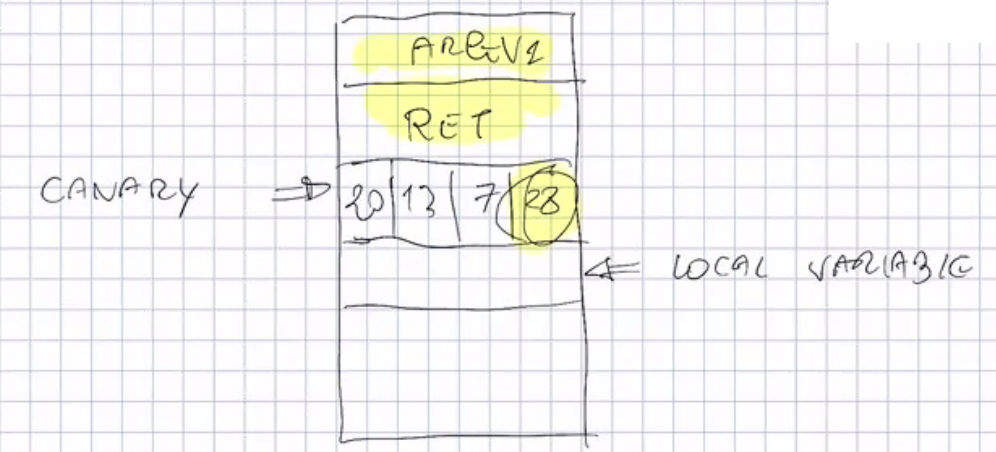
\includegraphics[scale = 0.5]{cattack}
\end{center}
To guess the canary we try every value from \emph{0 to 256} every byte, when the thread crashes we proceed with the next value, if the custom value doesn't invoke a crash, we found our value. Using this technique we can also guess the value of the return address.

\item Blind ROP: this technique remotely locates ROP gadgets (write functions)
The goal is to find enough gadgets to invoke \emph{write}. If we manage this, the binary can be dumped from memory to the network to find more gadgets. As previously mentioned, the \emph{write} system call takes 3 arguments: a socket, a buffer and a length. These are passed in \emph{rdi, rsi, rdx} registers, and the system call is stored in the \emph{rax} register. The following gadgets are therefore needed:
\begin{center}
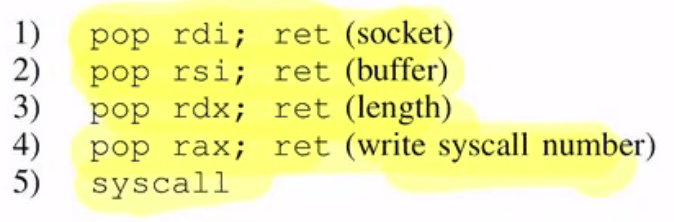
\includegraphics[scale = 0.5]{gadg}
\end{center}
\emph{but how do we find these gadgets?}\\
\emph{pop rdi, rsi, rdx} are manageable, \emph{pop rax and syscall} are the problematic functions, syscall is almost never called since this is usually done through libraries.\\
To effectively find gadgets, we modify progressively the return address, sorting them into crash gadgets, which cause the socket to crash, non-crash gadgets, which produce an arbitrary effect. 
\begin{center}
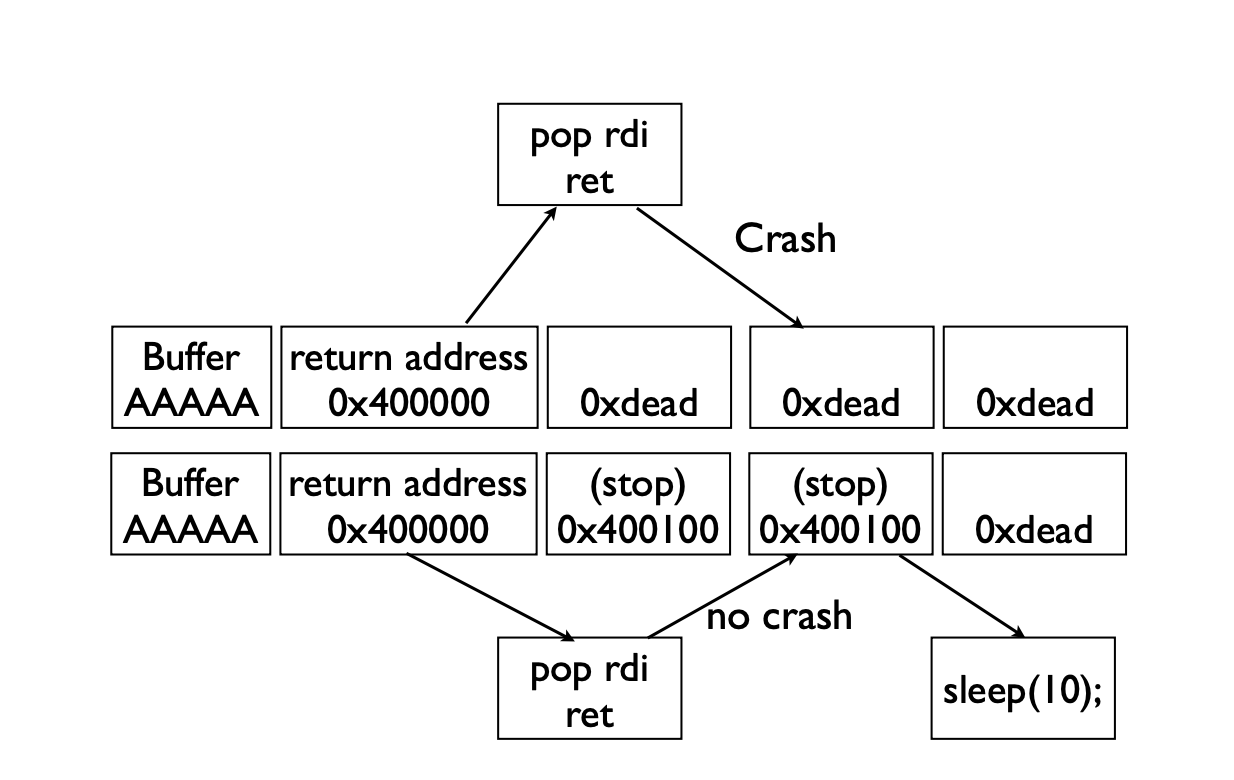
\includegraphics[scale = 0.5]{cgadg}
\end{center}
We further elaborate on non-crash gadgets, implementing probes, traps and stops. If the gadget produce the effect we want the stop is invoked and the gadget is selected.
\begin{center}
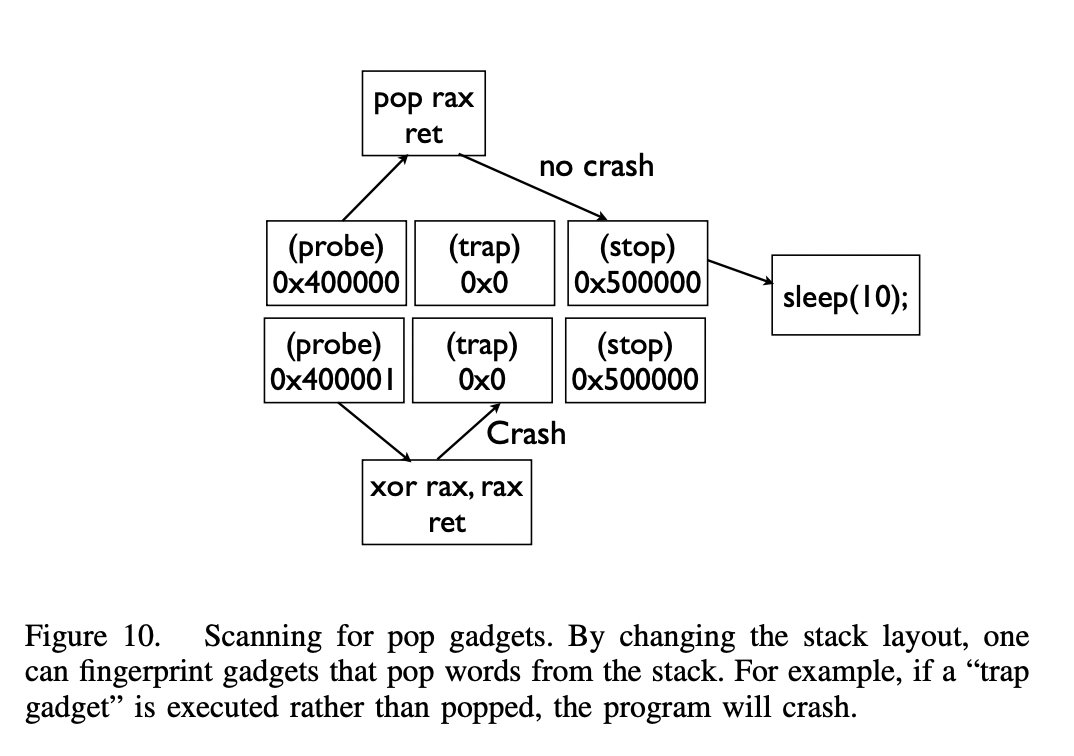
\includegraphics[scale = 0.4]{popstore}
\end{center}
\end{enumerate}
To call functions the PLT (static loader table) and GOT (populated by the dynamic linker) tables are used at runtime to find libraries.
\begin{center}
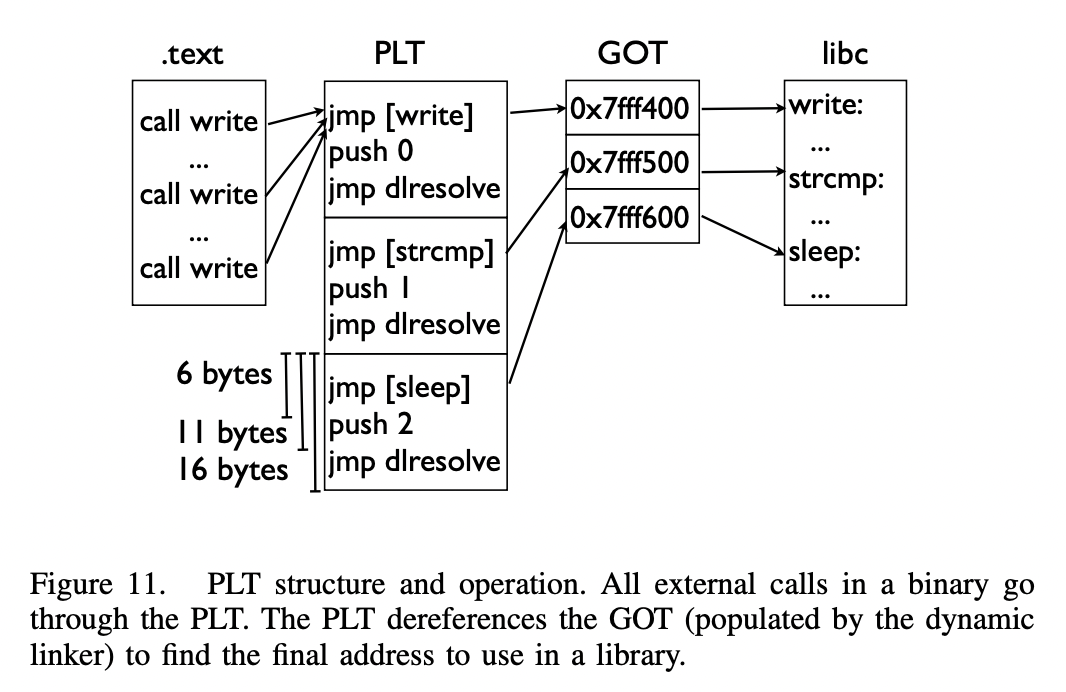
\includegraphics[scale = 0.4]{plt}
\end{center}
We have seen that memory safety and type safety solve most of the memory errors, \emph{control flow integrity} is the last passive defence mechanism we see.\\

\section*{Control flow integrity}
CFI aims to defend a program by observing the program's behaviour, if the program is not doing what we expect it to do, it might be compromised. To do this we need to define an \textbf{expected behaviour}, create mechanisms which let us \textbf{detect deviations from expectations effectively}, implement policies which \textbf{prevent compromise of the detector}
\subsection*{Control flow graph | CFG} to define expected behaviour.
One way we can do this is by utilising \textbf{call graphs}. The aim is to represent all the possible combinations of function calls to other functions
\begin{center}
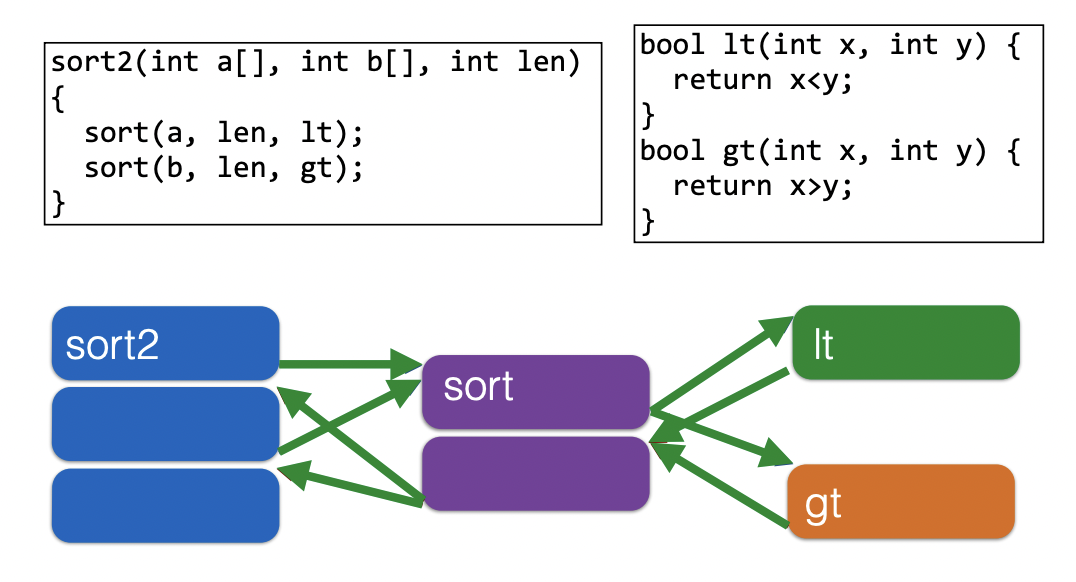
\includegraphics[scale = 0.4]{cfi}\\
\emph{example of a function which sorts by calling 2 distinct functions}
\end{center}
The code is broken up into \textbf{basic blocks}, \textbf{calls} are distinguished from \textbf{returns.}


\subsection*{In-line reference monitor | IRM} to detect deviations from expectations, it works by introducing control methods inside the program (in binary or inside the program)
\subsection*{Sufficient randomness and immutability} to avoid compromise of the detector\\\\
\emph{So how efficient is CFI actually?}\\
Classic CFI imposes a 16\% overhead on average, 45\% in the worst cases, it works on arbitrary executables, and is not modular.\\
Modular CFI imposes a 5\% overhead on average, and 12\%in the worst cases, it works only in C (part of the LLVM, source code), and is modular, with separate compilation routines\\\\
\emph{And how secure is CFI actually?}\\
MFI can eliminate 95\% of ROP gadgets on x86-64 versions of SPEC2006 benchmark suites. Average indirect-target reduction is of $>99\%$, meaning that the percentage of possible targets of indirect jumps is almost completely ruled out.

\end{document}  
